\subsection{Frostbite}
We will now review the results of testing in the Frostbite game, another game of the Atari 2600. A frame form the game is shown in Figure~\ref{fig:frostbite_frame}. In this game a character has to collect ice to build an igloo. The bottom two thirds of the screen are covered by a mass of water with four rows of ice blocks floating horizontally. The player moves by jumping from one row to another while trying to avoid various kinds of foes including crabs and birds. There are also fish which grant extra points. On the top of the screen is the shore where the player must build the Igloo. From the fourth level onwards there is also a polar bear walking around on the shore which must be avoided. Each time the player jumps on a piece of ice in a row its color changes from white to blue and the player gets an ice block in the Igloo on the shore. The player has the ability to change the direction in which the ice is flowing by pressing the fire button, but that costs a piece of the Igloo.\par
\begin{figure}
 \centering 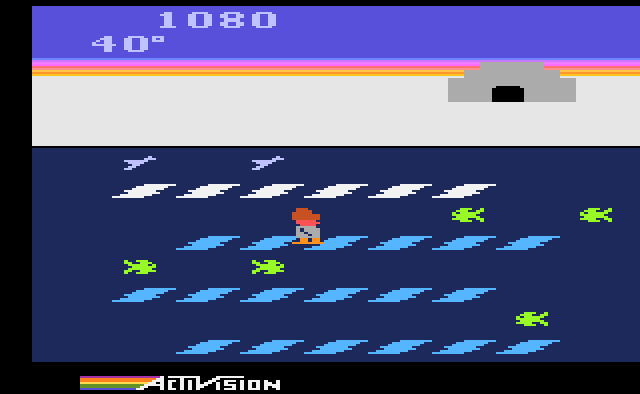
\includegraphics[width=0.7\linewidth]{frostbite_frame.png}
 \caption{Frame taken from the game Frostbite.}
 \label{fig:frostbite_frame}
\end{figure}
After the player has jumped on all the pieces on the screen, they all turn back to white and one can jump on them again. When all the 15 ice blocks required for building the Igloo are gathered, the player has to get back to the shore and get inside it, thus proceeding to the next level. On every level the enemies and the ice blocks move slightly faster than in the previous level making the game more difficult.\par
Each level must be completed in 45 seconds, (represented as the declining temperature,) else the player dies frozen. The faster the level is completed the more bonus points are awarded to the player.\par
Figure~\ref{fig:frostbite_learning_curve} shown the results of our tests
\begin{figure}
 \centering 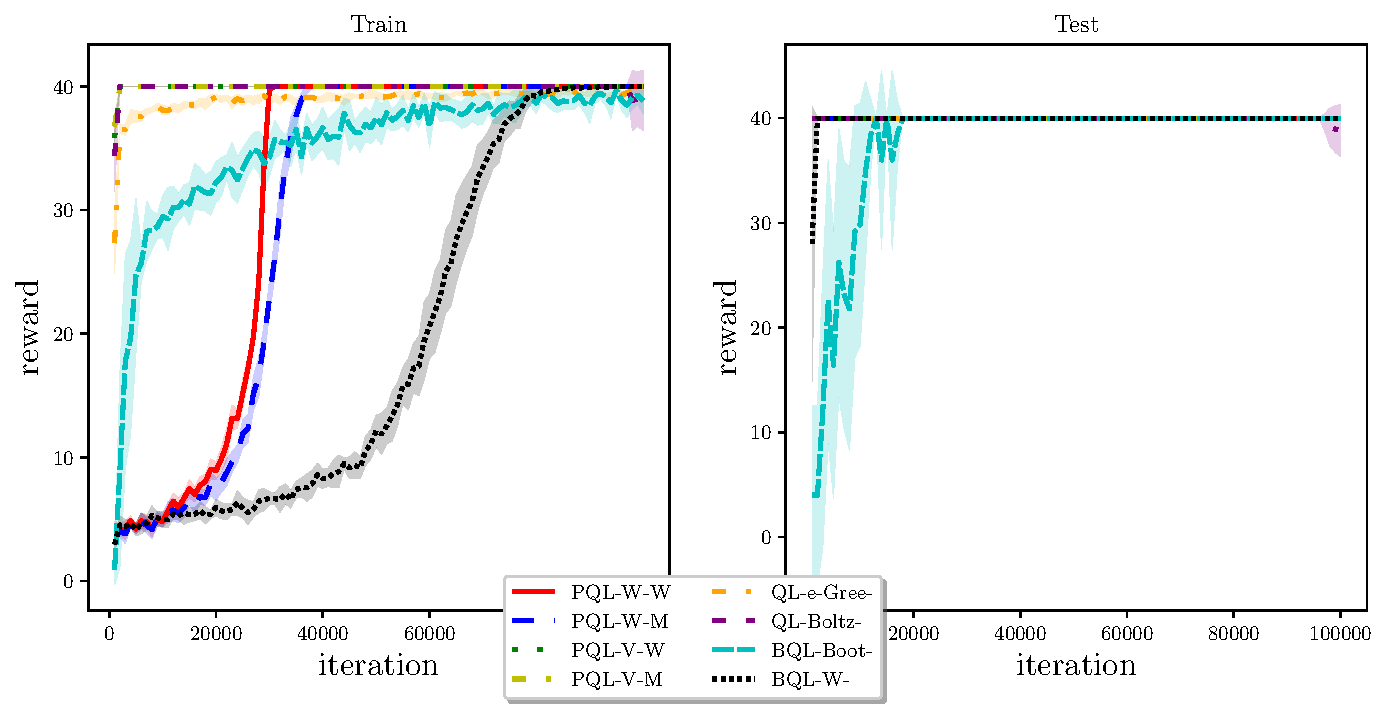
\includegraphics[width=\linewidth]{Frostbite/learning_curve.pdf}
 \caption{Evaluation scores in Frostbite.}
 \label{fig:frostbite_learning_curve}
\end{figure}